\documentclass{beamer}
\usetheme{Madrid}

\usepackage[utf8]{inputenc}
\usepackage[T1]{fontenc}
\usepackage[magyar]{babel}
\usepackage{graphicx}
\usepackage{booktabs}
\usepackage{multicol}
\usepackage{caption}
\usepackage{amsmath}
\usepackage{xcolor}
\usepackage{listings}

% saját package-ek
\usepackage{amssymb}
\usepackage{multirow}
\usepackage{hyperref}

\definecolor{mygreen}{rgb}{0,0.6,0}
\definecolor{mygray}{rgb}{0.5,0.5,0.5}
\definecolor{mymauve}{rgb}{0.58,0,0.82}

\title{\bf Nyelvi modellek teljesítményének összehasonlítása egy kontextusalapú szójelentés-felismerés (Word-in-Context) probléma megoldására és saját kiértékelő rendszer fejlesztése Pythonban}


\author{Fábián Bernát}
\institute{Programtervező Informatikus BSc\\Szegedi Tudományegyetem}
\date{2025}

\begin{document}
    \frame{\titlepage}

    \begin{frame}{Probléma}
        \begin{itemize}
            \item A természetes nyelvekben sok a többjelentésű szó. A statikus szóbeágyazások képtelenek tükrözni a szavaknak ezt a dinamikus természetét
            \item Számtalan kisméretű nyelvi modell létezik, ám nincs olyan átfogó összehasonlítás teljesítményükről, mint az \href{https://lmarena.ai/}{LMArena} platformon
        \end{itemize}
    \end{frame}

    \begin{frame}{A WiC feladat}
        \begin{itemize}

            \item Egy többjelentésű szó két különböző mondatban.
            \item Döntés: ugyanazt jelenti-e a szó? Igen/Nem - bináris osztályozás
            \item \textbf{Adatformátum:} célszó <tab> szófaj címke <tab> index1-index2 <tab> példamondat\_1 <tab> példamondat\_2
            \item Pl.: \textit{"Fix your eyes on this spot." <-> "Fix a race."}
            \item $\sim7500$ példa szétosztva tanító-, validációs- és teszthalmazra (73-8-19\%)
        \end{itemize}
    \end{frame}


    \begin{frame}{Kutatási célok}
        \begin{itemize}
            \item \textbf{Fő célkitűzések:}
            \begin{itemize}
                \item Kontextuális szóbeágyazási technikák és generatív modellek képességeinek feltárása
                \item Különböző nyelvi modellek
                \begin{itemize}
                    \item pontosságának összehasonlítása a WiC feladaton determinisztikus és izolált módon
                    \item konzisztenciájának összehasonlítása
                \end{itemize}
                \item Saját kiértékelő rendszer fejlesztése legalább 60\%-os pontossággal
            \end{itemize}
        \end{itemize}
    \end{frame}

    \begin{frame}{Használt technológiák és platformok}

        A modellek összehasonlításához:
        \begin{itemize}
            \item Google Colab és PyCharm, Python futtatókörnyezet
            \item Git, GitHub
            \item LMArena, Hugging Face
            \item CUDA, Accelerate, Transformers, BERT
            \item Google Táblázatok, Apps Script
        \end{itemize}
        A kiértékelő rendszerhez:
        \begin{itemize}
            \item NLTK WordNet szinonimahalmazok – szóértelmezéshez

            \item SentenceTransformer – BERT-alapú mondatembeddinghez

            \item TF-IDF – szövegösszehasonlításhoz %, cosine\_similarity

%\item scikit-learn – küszöboptimalizálás, értékelés, tévesztési mátrix
            \item MatPlotLib, SeaBorn - Ábrákhoz
        \end{itemize}
    \end{frame}

    \begin{frame}{Miért bontottam ketté?}

        Mik a fő különbségek a Google Colab-os és a lokális Python megoldás között?
        \begin{itemize}
            \item A \textbf{Colab szkript} távoli gép erőforrásait (pl. GPU-t) használja, nem terheli a saját számítógépet\\
            \item Következtető , auto-regresszív modellek (GPT-szerűek)
            \item Absztraktabb, magasabb szintű mondatértelmezés a szavak szétbontása helyett \\
            \item  Bármilyen szöveg beadható inputként, nem csak a WiC adathalmazban szereplő formátumú, tabulált szöveg
            \vspace*{0.3cm}
            \item A \textbf{lokális Python projekt} gyorsabb, biztonságosabb és elérhető a fájlrendszer, készíthetők ideiglenes fájlok\\
            \item BERT-típusú modellek és hagyományosabb módszerek\\
            \item Jobb konfigurálhatóság
        \end{itemize}

    \end{frame}


    \begin{frame}{Hugging Face modellek futtatása Google Colab notebookban}
        188 db \textbf{determinisztikus} és \textbf{izolált} válasz\\  Hogyan \textbf{izolálom} a válaszadásokat? \\
        \begin{itemize}
            \item A kérdések egy Python szótárban\\
            \item Egy \texttt{foreach} ciklusban végigiterálok az összes kérdésen, majd mivel ezek chat modellek, minden iteráció után törlődik a modell memóriája, így nem befolyásolja a következő válaszadás(oka)t\\
        \end{itemize}
        Mitől lesz \textbf{determinisztikus}?\\
        \begin{itemize}
            \item Az előtanított modell betöltése közben paraméter beállítása gondoskodik róla, hogy ne legyen véletlenszerűség a válaszban, így egy adott inputra mindig ugyanaz a modell válasza, függetlenül a futtatások számától\\
        \end{itemize}

    \end{frame}

    \begin{frame}{Modellek eredményeinek eltárolása Google táblázatban}
        \begin{figure}
            \centering
            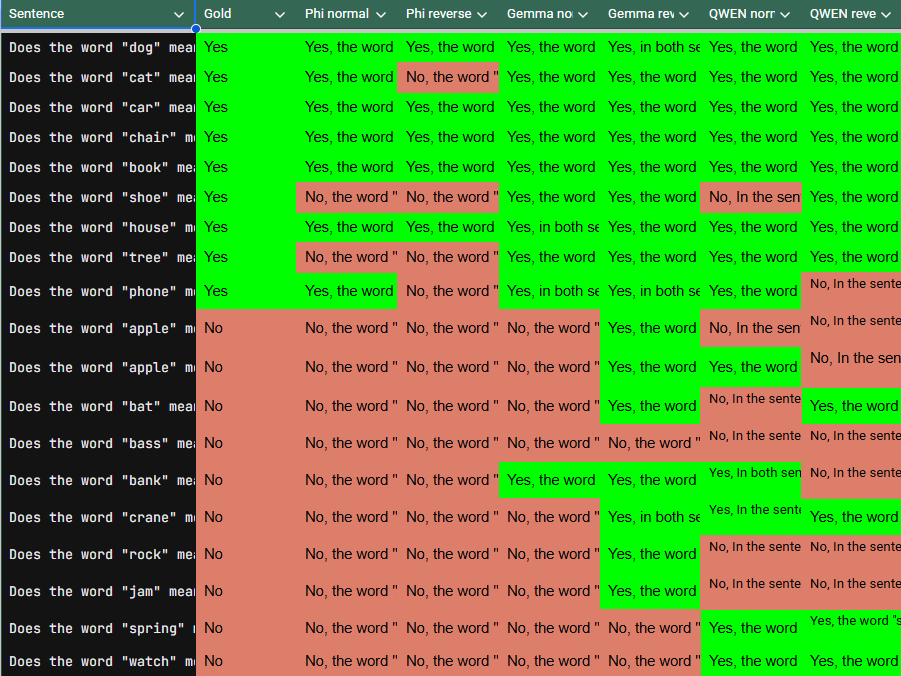
\includegraphics[width=0.75\linewidth]{konnyu-kerdesek-eredmenyei.png}
            \label{fig:enter-label}
        \end{figure}
    \end{frame}

    \begin{frame}{Hugging Face modellek eredményeinek összehasonlítása}
        \begin{table}[H]
            \centering
            \label{tab:model-eval-summary}
            \resizebox{\textwidth}{!}{
                \begin{tabular}{|c|c|c|c|c|c|}
                    \hline
                    \textbf{Modell} & \textbf{Nehézség} & \textbf{Pontosság (\%)} & \textbf{Kiegy. Pontosság (\%)} & \textbf{Egyezés (\%)} & \textbf{Megjegyzés} \\
                    \hline
                    \multirow{6}{*}{Phi}
                    & Közepes N & 53.33 & 56.03 & \multirow{2}{*}{95.00} &Legjobb egyezés, de alacsony pontosság \\
                    & Közepes F & 58.33 & 60.71 & & \\
                    \cline{2-3}\cline{5-6}
                    & Nehéz N   & 53.33 & 44.44 & \multirow{2}{*}{60.00} &  \\
                    & Nehéz F   & 60.00 & 52.78 & & Válasza szinte minden kérdésre "nem" \\
                    \hline
                    \multirow{6}{*}{Gemma}
                    & Közepes N & 60.00 & 61.83 & \multirow{2}{*}{85.00} & Legpontosabb közepesekre \\
                    & Közepes F & 55.00 & 56.47 & & \\
                    \cline{2-3}\cline{5-6}
                    & Nehéz N   & 68.75 & 72.22 & \multirow{2}{*}{73.33} & \\
                    & Nehéz F   & 60.00 & 55.56 & & Legjobb nehéz kérdéseken is \\
                    \hline
                    \multirow{6}{*}{Qwen}
                    & Közepes N & 56.67 & 57.37 & \multirow{2}{*}{91.67} & Erős egyezés \\
                    & Közepes F & 58.33 & 58.93 & &  \\
                    \cline{2-3}\cline{5-6}
                    & Nehéz N   & 46.67 & 52.78 & \multirow{2}{*}{80.00} & \\
                    & Nehéz F   & 40.00 & 50.00 & & Válasza szinte minden kérdésre "igen" \\
                    \hline
                \end{tabular}
            }
            \caption{A három nyelvi modell teljesítménye különböző kérdésnehézségek és sorrendek mentén. N=normál, F=fordított}
        \end{table}
    \end{frame}

    \begin{frame}{Saját adatfeldolgozó és kiértékelő rendszer fejlesztése}
        \begin{itemize}
            \item \textbf{Implementáció:} PyCharm, Python 3.12
            \item \textbf{Rendszer célja:} A WiC adathalmaz feldolgozása
            \item \textbf{Fejlesztési módszer:} Inkrementális modell
        \end{itemize}
        \begin{itemize}
            \item \textbf{Kiértékelési módszerek:}
            \begin{itemize}
                \item Pontosság (Accuracy)
                \item Tévesztési mátrix
            \end{itemize}
            \item \textbf{Tévesztési mátrix elemei:}
            \begin{itemize}
                \item TP: Helyesen felismert jelentésazonosság
                \item FP: Tévesen azonosnak vélt jelentések
                \item FN: Fel nem ismert jelentésazonosság
                \item TN: Helyesen felismert jelentéskülönbség
            \end{itemize}
        \end{itemize}
    \end{frame}



    \begin{frame}{Saját rendszer eredményei}
        \begin{table}[h]
            \centering
            \begin{tabular}{c|c|c|c}
                \hline
                Adathalmaz & Mód & Pontosság (\%) & Futásidő (másodperc) \\ \hline
                train & all-MiniLM-L6-v2 & 59.912 & 8294.84 \\ \hline
                train & TF-IDF & 57.970 & 5903.44 \\ \hline
                dev & all-MiniLM-L6-v2 & 60.696 & 128.44 \\ \hline
                dev & TF-IDF & 62.088 & 91.95 \\ \hline
                test & all-MiniLM-L6-v2 & 59.571 & 382.36 \\ \hline
                test & TF-IDF & 60.658 & 332.65 \\ \hline
            \end{tabular}
            \caption{A \texttt{wic\_tfidf\_or\_sensebert\_baseline\_single.py} eredményei és futásideje a különböző beállítások mellett.
            }
            \label{tab:my_label}
        \end{table}
    \end{frame}

% desc      Az egyszerűbb kérdéseket tartalmazó train halmazon a BERT jobban teljesít, míg a nehezebb kérdésekből álló dev és test esetén a TF-IDF minimálisan pontosabb. Ez alapján leszűrhető, hogy a BERT módszer egyszerűbb kérdések esetén hasznosabb, főleg ha nem lényeges a gyors a futásidő.

    \begin{frame}{Eredmények 3/3}
    {\bf Tévesztési mátrixok}
    {\centering

% első sor: kettő egymás mellett
        \begin{minipage}{0.32\linewidth}
            \centering
            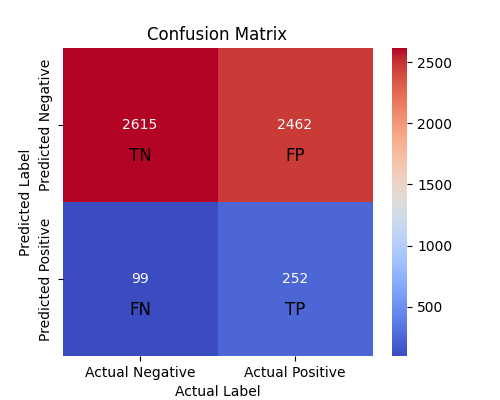
\includegraphics[width=\linewidth]{graphics/WiC_confusion_matrix_abra.train.png}\\
            \small Train halmaz
        \end{minipage}
        \begin{minipage}{0.32\linewidth}
            \centering
            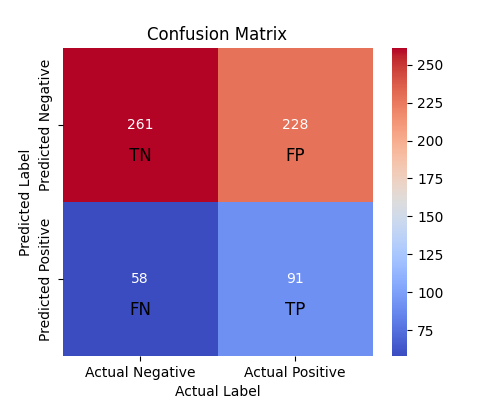
\includegraphics[width=\linewidth]{graphics/WiC_confusion_matrix_abra.dev.png}\\
            \small Dev halmaz
        \end{minipage}
        \begin{minipage}{0.32\linewidth}
            \centering
            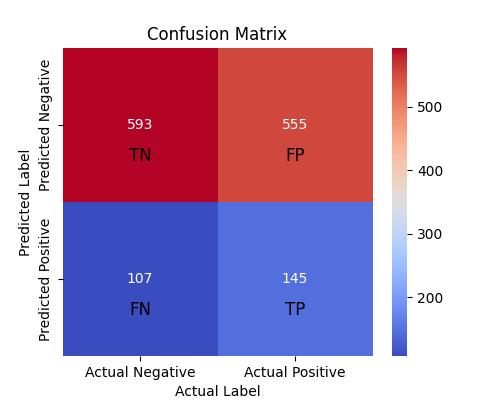
\includegraphics[width=\linewidth]{graphics/WiC_confusion_matrix_abra.test.png}\\
            \small Test halmaz
        \end{minipage}

        \vspace{0.25cm}
        \captionof{figure}{A TF-IDF megoldás tévesztési mátrixai a train, dev és test halmazra}
        \label{fig:enter-label5}
    }
    \end{frame}



    \begin{frame}{Megfigyelések és tanulságok}
        \begin{itemize}
            \item A Gemma jobban teljesített a WiC feladatra, mint a Phi vagy a QWEN modell, de vannak alternatívák
            \item A modell mérete és a pontosság közötti összefüggés nem mindig lineáris
            \item Legkonzisztensebb: Gemini-2.5, GPT-4, GPT-4.5o
            \item A Gemini 2.5 Pro túlteljesített minden megvizsgált modellt, 80\% pontosság, de nem izolált és nem determinisztikus
            \item TF-IDF- és BERT-alapú osztályozó rendszer: $\sim60$\%
        \end{itemize}
    \end{frame}

    \begin{frame}{Összegzés}
        \begin{itemize}
            \item \large{WiC probléma}
            \item \large{Legkonzisztensebb nagy nyelvi modellek megtalálása}
            \item \large{A Phi, Gemma és a QWEN összehasonlítása}
            \item \large{Saját kiértékelő rendszer fejlesztése}
        \end{itemize}
        \vspace{1cm}
        \small{Témavezető: Berend Gábor}
    \end{frame}

\end{document}
